\section{Étude des solutions potentielles (avant choix final)}
Avant de stabiliser la solution, plusieurs options ont été évaluées, en cohérence avec les contraintes du projet : rapidité de développement, possibilité d’évolution (vers e-commerce), simplicité de maintenance et autonomie de l’artisane.

\subsection{Option 1 : site vitrine statique (CMS ou générateur)}
Une première approche consistait à produire un site principalement statique (WordPress, Webflow, ou générateur statique). Cette option présente des avantages (mise en ligne rapide, administration “contenu”), mais atteint rapidement ses limites dès qu’on introduit :
\begin{itemize}
    \item des règles métier (créneaux de rendez-vous, disponibilité par service) ;
    \item un back-office sur mesure (tri d’images, gestion des statuts) ;
    \item une base de données relationnelle cohérente.
\end{itemize}
Elle a donc été jugée insuffisante pour un besoin évolutif.

\subsection{Option 2 : architecture séparée Front + Back}
Une seconde approche envisageait un front (React) et un back séparé (Express/NestJS ou Django/FastAPI). Cette option est robuste, mais elle augmente le coût d’infrastructure et la charge de maintenance (deux projets, deux déploiements, plus de configuration). Pour RUHENNA, une solution monolithique Next.js est apparue plus adaptée.

\subsection{Option retenue : Next.js full-stack + Prisma + PostgreSQL}
La solution finale combine l’interface (front public et back-office) et l’API dans une seule application Next.js, avec Prisma pour le modèle de données et PostgreSQL (Neon) pour le stockage, afin d’obtenir une base saine et une mise en production simple sur Vercel.

\section{Solution implémentée : architecture et composants}

\subsection{Vue d’ensemble technique}
La plateforme est structurée autour de quatre blocs :
\begin{itemize}
    \item \textbf{Front public} : pages accessibles aux visiteurs (vitrine, galerie, blog, boutique, réservation, contact) ;
    \item \textbf{Back-office} : pages \texttt{/admin} pour gérer le contenu et les demandes ;
    \item \textbf{API} : endpoints REST via les Route Handlers Next.js (\texttt{/api/...}) ;
    \item \textbf{Données et médias} : PostgreSQL (Neon) via Prisma, et Cloudinary pour les images.
\end{itemize}

\begin{figure}[H]
    \centering
    \begin{tikzpicture}[
        node distance=10mm,
        box/.style={draw, rounded corners, align=center, inner sep=7pt, text width=0.30\textwidth},
        arrow/.style={-{Stealth[length=2.2mm]}, thick}
    ]
    \node[box] (public) {\textbf{Navigateur (public)}\\\small Pages \texttt{src/app/(main)}\\\small \texttt{/boutique}, \texttt{/galerie}, \texttt{/reservation}, ...};
    \node[box, right=of public] (api) {\textbf{API Next.js}\\\small \texttt{src/app/api/*/route.ts}\\\small validation, règles métier};
    \node[box, right=of api] (db) {\textbf{PostgreSQL (Neon)}\\\small Prisma Client\\\small données persistées};
    \node[box, below=of public] (admin) {\textbf{Navigateur (admin)}\\\small Pages \texttt{src/app/admin}\\\small gestion CRUD + tri};
    \node[box, below=of api] (cloud) {\textbf{Cloudinary}\\\small stockage et CDN images\\\small upload via \texttt{/api/upload}};
    \draw[arrow] (public) -- (api);
    \draw[arrow] (admin) -- (api);
    \draw[arrow] (api) -- (db);
    \draw[arrow] (api) -- (cloud);
    \end{tikzpicture}
    \caption{Architecture applicative : Next.js centralise UI et API, Prisma relie l’application à PostgreSQL, Cloudinary gère les médias.}
    \label{fig:architecture_tikz}
\end{figure}

\subsection{Structure du dépôt et conventions Next.js}
Le code suit l’architecture par conventions de Next.js (App Router). Les dossiers principaux sont :
\begin{itemize}
    \item \texttt{src/app/} : pages, layouts, et endpoints API ;
    \item \texttt{src/components/} : composants UI réutilisables (header/footer, éditeur, uploaders, etc.) ;
    \item \texttt{src/lib/} : accès DB, validation, configuration Cloudinary, utilitaires ;
    \item \texttt{prisma/} : schéma Prisma, migrations, seed et ERD.
\end{itemize}

\subsection{Routage : pages publiques, administration et API}
Trois familles de routes coexistent :
\begin{enumerate}
    \item \textbf{Routes publiques} : \texttt{src/app/(main)/...} (ex. \texttt{/boutique}, \texttt{/blog}).
    \item \textbf{Routes admin} : \texttt{src/app/admin/...} (ex. \texttt{/admin/produits}, \texttt{/admin/blog}).
    \item \textbf{Routes API} : \texttt{src/app/api/.../route.ts} (ex. \texttt{/api/contact}, \texttt{/api/rendez-vous}).
\end{enumerate}

\section{Base de données : schéma, entités, relations}

\subsection{Rôle de Prisma (ORM)}
Prisma agit comme une couche intermédiaire entre l’application et PostgreSQL. Les modèles sont définis dans \texttt{prisma/schema.prisma} et Prisma génère un client typé, utilisé dans les pages serveur et les routes API.

\subsection{ERD (diagramme entité-association)}
Le diagramme ERD a été généré à partir du schéma Prisma. Il permet d’illustrer les principales entités (\textit{produits, catégories, services, rendez-vous, blog, messages, images}) et les liens entre elles.

\begin{figure}[H]
    \centering
    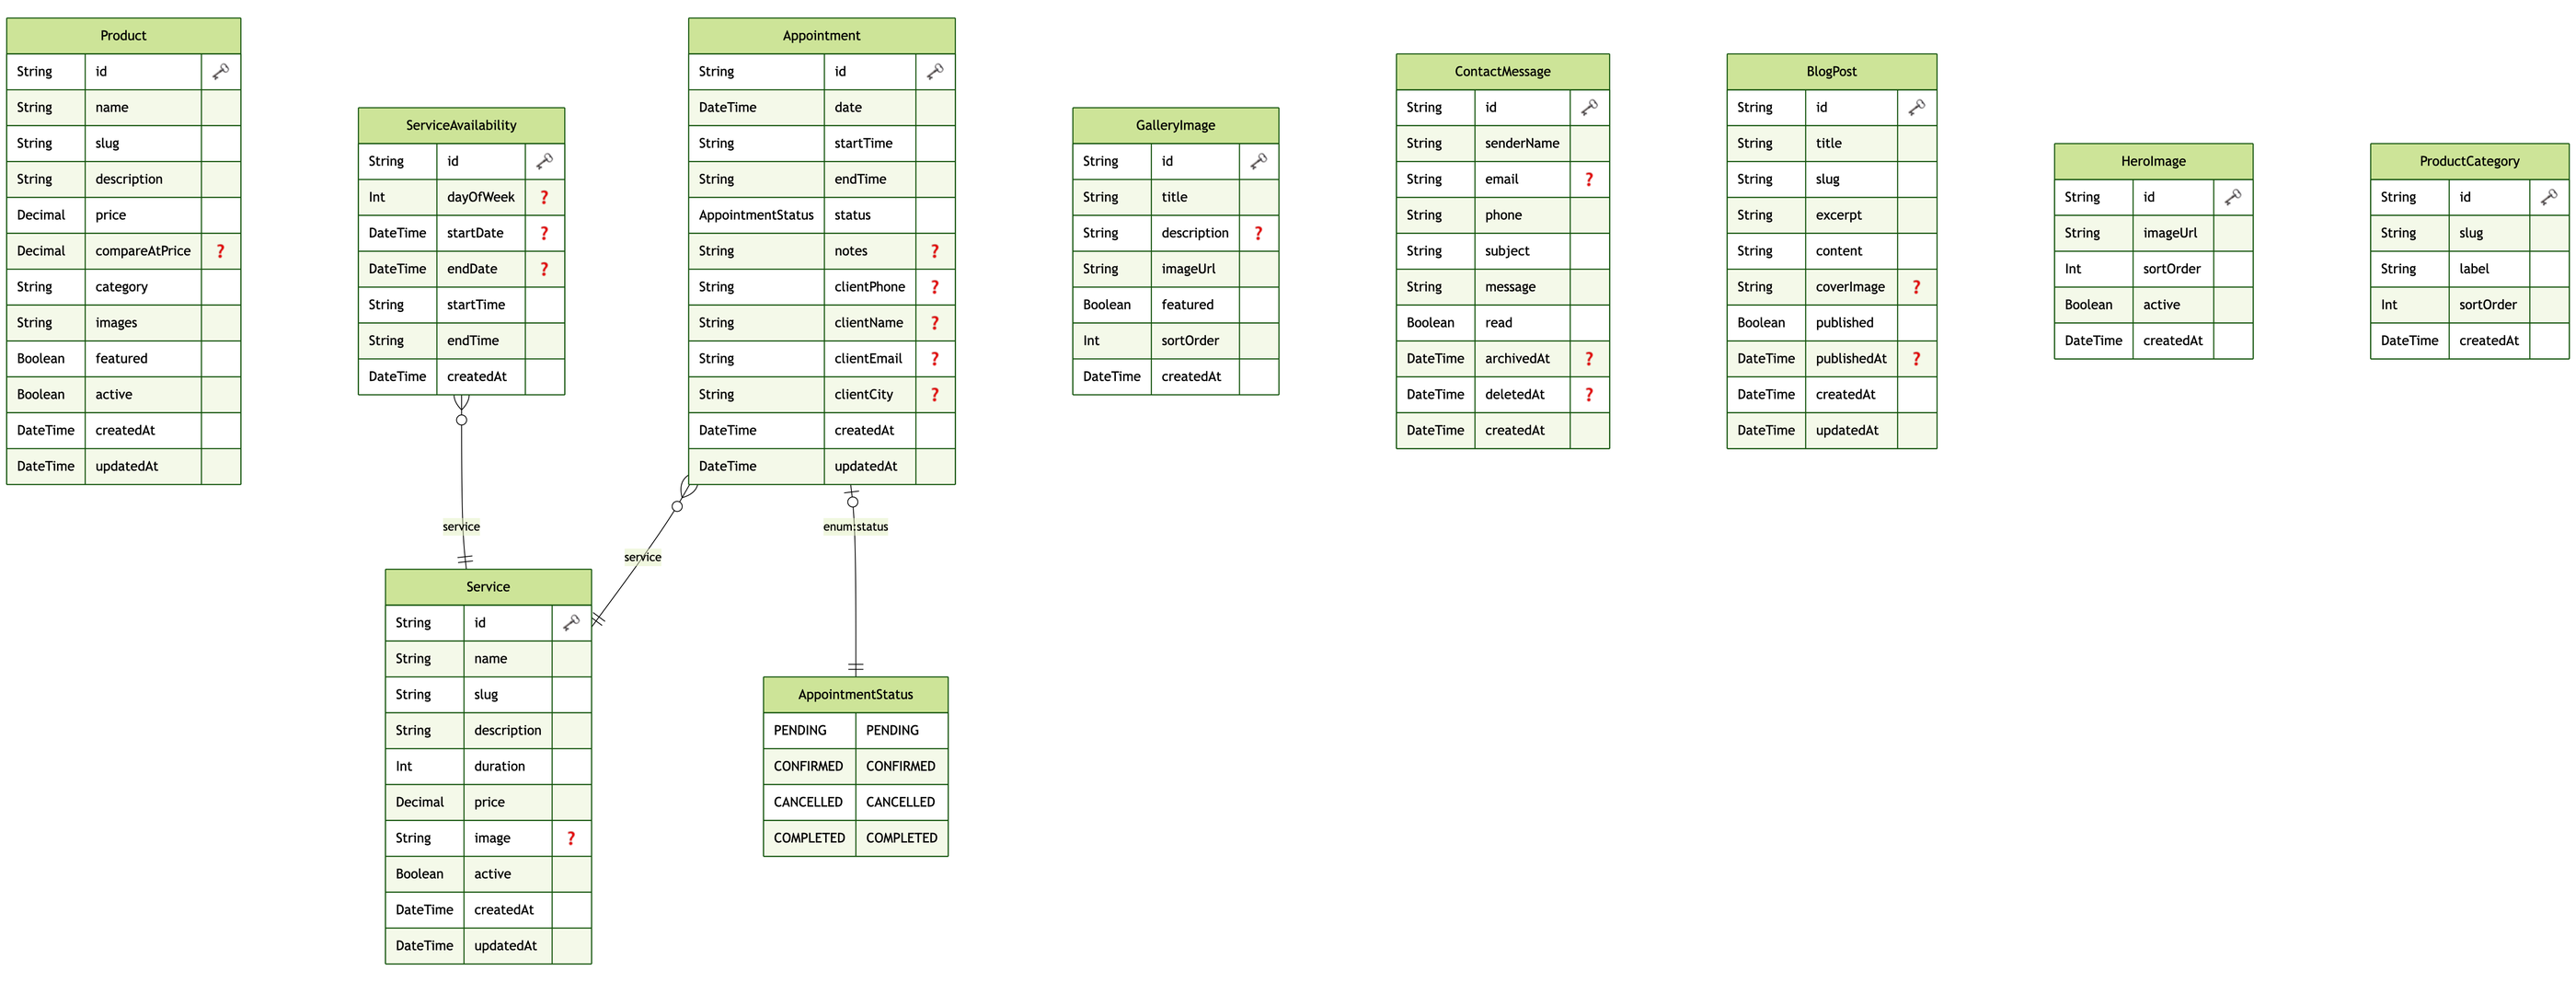
\includegraphics[width=\textwidth]{Figures/ERD.png}
    \caption{ERD de la base de données RUHENNA (généré depuis \texttt{prisma/schema.prisma}).}
    \label{fig:erd}
\end{figure}

\subsection{Modèle de données}
Le modèle de données s’organise autour d’entités qui correspondent directement aux besoins du site (catalogue, réservation, contenu, médias, messages) :
\begin{itemize}
    \item \textbf{Produits} (\texttt{Product}) : nom, description, prix, catégorie, liste d’URLs d’images (Cloudinary), statut actif/mis en avant.
    \item \textbf{Catégories} (\texttt{ProductCategory}) : liste ordonnée (champ \texttt{sortOrder}) pour maîtriser l’affichage de la boutique.
    \item \textbf{Services} (\texttt{Service}) : durée et prix, associés à des règles de disponibilité (\texttt{ServiceAvailability}).
    \item \textbf{Rendez-vous} (\texttt{Appointment}) : date, heure de début/fin, statut (en attente, confirmé, annulé, terminé).
    \item \textbf{Blog} (\texttt{BlogPost}) : titre, slug, extrait, contenu HTML, image de couverture, publication.
    \item \textbf{Messages} (\texttt{ContactMessage}) : informations du demandeur et contenu, avec gestion “lu / archivé / supprimé”.
    \item \textbf{Médias} : images de galerie et de bannière (\texttt{GalleryImage}, \texttt{HeroImage}) avec ordre d’affichage.
\end{itemize}

Pour éviter deux rendez-vous au même horaire, une contrainte d’unicité impose qu’à une date donnée, un même \texttt{startTime} ne puisse pas être réservé deux fois. Lors de la création d’un rendez-vous, l’application vérifie aussi l’absence de \textbf{chevauchement} horaire avec les rendez-vous déjà enregistrés.

\section{Fonctionnalités du front public}

\subsection{Page d’accueil et identité de marque}
La page d’accueil combine :
\begin{itemize}
    \item un \textbf{hero} avec carrousel d’images (\texttt{HeroImage}) ;
    \item une mise en avant des réalisations (\texttt{GalleryImage.featured}) ;
    \item des appels à action (galerie et réservation).
\end{itemize}
Le choix d’une page d’accueil dynamique permet de publier rapidement de nouvelles réalisations, sans redeployer manuellement des assets.

\subsection{Catalogue (boutique) : logique de lecture}
La boutique est conçue comme un \textbf{catalogue} : les produits sont consultables, filtrables par catégories, et la prise de commande passe par le contact (pas de paiement intégré à ce stade). Cette approche correspond à une phase où l’offre évolue et où l’artisane souhaite conserver un lien direct avec la clientèle.

\subsection{Galerie : consultation}
La galerie propose une grille responsive afin de mettre en valeur les réalisations, sans ajouter de complexité inutile dans le parcours utilisateur.

\subsection{Blog : contenu riche et SEO}
Les articles sont stockés en base (table \texttt{BlogPost}) et publiés/dépubliés via l’administration.

\section{Système de réservation : calcul de créneaux et création d’un rendez-vous}

\subsection{Parcours utilisateur (5 étapes)}
Le formulaire de réservation est conçu en plusieurs étapes (service, date, horaire, informations, récapitulatif) afin de réduire les erreurs et de guider la saisie.

\subsection{Calcul des créneaux disponibles (API)}
L’endpoint \texttt{/api/rendez-vous/slots} calcule les créneaux à partir :
\begin{itemize}
    \item de la durée du service ;
    \item des règles \texttt{ServiceAvailability} ;
    \item des rendez-vous existants non annulés (détection de chevauchement).
\end{itemize}

\subsection{Création d’une demande de rendez-vous}
Une fois un créneau choisi, \texttt{/api/rendez-vous} crée un enregistrement \texttt{Appointment} en statut \texttt{PENDING}. L’API vérifie :
\begin{itemize}
    \item la validité du payload (\textbf{Zod}) ;
    \item l’existence du service ;
    \item la non-disponibilité du créneau (conflit).
\end{itemize}

Le navigateur envoie un JSON minimal à l’API, avec notamment :
\begin{itemize}
    \item \texttt{serviceId} : \textit{"ck..."}
    \item \texttt{date} : \textit{"AAAA-MM-JJ"}
    \item \texttt{startTime} : \textit{"11:00"}
    \item \texttt{name/email/phone/city} : informations de contact
\end{itemize}
Si tout est valide, l’API crée un rendez-vous \textbf{en attente} et renvoie un identifiant de suivi. Si le créneau est pris entre-temps, elle renvoie un message “créneau indisponible”.

\section{Formulaire de contact : validation et stockage}

\subsection{API de contact}
La route \texttt{/api/contact} illustre l’utilisation de Zod pour valider l’entrée et de Prisma pour persister le message.
Un message “Demande de devis” contient des champs simples (nom, email, sujet, message). Si un champ est mal formé (email invalide, message trop court), la réponse contient une liste d’erreurs \textit{par champ}, ce qui permet d’afficher une aide claire à l’utilisateur.

\section{Communication entre l’interface React et l’API}
Les formulaires (contact, réservation, administration) sont des composants React côté navigateur (\textit{Client Components}). Ils envoient des requêtes HTTP à l’API (\texttt{/api/...}), qui valide les données (Zod), puis appelle Prisma pour écrire/lire dans PostgreSQL.

\begin{figure}[H]
    \centering
    \begin{tikzpicture}[
        node distance=10mm,
        box/.style={draw, rounded corners, align=center, inner sep=7pt, text width=0.28\textwidth},
        arrow/.style={-{Stealth[length=2.2mm]}, thick}
    ]
    \node[box] (ui) {React (navigateur)\\\small formulaire + \texttt{fetch}};
    \node[box, right=of ui] (api2) {API Next.js\\\small validation + règles};
    \node[box, right=of api2] (db2) {PostgreSQL\\\small via Prisma};
    \draw[arrow] (ui) -- node[above]{\small JSON} (api2);
    \draw[arrow] (api2) -- node[above]{\small requêtes} (db2);
    \draw[arrow] (api2) -- node[below]{\small réponse JSON} (ui);
    \end{tikzpicture}
    \caption{Flux simplifié : UI React $\rightarrow$ API $\rightarrow$ base de données.}
    \label{fig:react_api_flow}
\end{figure}
Le formulaire “Contact” construit un objet JSON avec les champs saisis, puis l’envoie à \texttt{/api/contact}. L’API répond soit :
\begin{itemize}
    \item \textbf{Succès} : \texttt{\{ success: true \}} + message de confirmation ;
    \item \textbf{Erreurs} : \texttt{\{ success: false, errors: ... \}} pour afficher les champs à corriger.
\end{itemize}

\subsection{Validation des formulaires avec Zod}
Zod sert à décrire ce qui est attendu (types, formats, longueurs) et à refuser des données incohérentes \cite{zodDocs}. Les erreurs sont \textbf{structurées} et donc faciles à afficher côté interface.

Dans le cas d’une réservation, si l’objet reçu ne respecte pas la structure attendue (date qui n’est pas au format \texttt{AAAA-MM-JJ}, email invalide, nom trop court), la validation échoue et renvoie des erreurs associées aux champs, comme :
\begin{itemize}
    \item \texttt{date} : “format de date invalide” ;
    \item \texttt{email} : “adresse email invalide” ;
    \item \texttt{name} : “au moins 2 caractères”.
\end{itemize}
De la même façon, si un champ obligatoire manque (par exemple \texttt{serviceId}) ou si un champ n’a pas le bon type, la requête est rejetée avant toute écriture en base.

\subsection{Éditeur de contenu riche (TipTap) pour le blog}
Le back-office propose un éditeur riche basé sur TipTap \cite{tiptapDocs}. Concrètement :
\begin{itemize}
    \item l’artisane écrit avec des outils (titres, listes, gras, images, liens) ;
    \item le contenu est enregistré en base sous forme de \textbf{HTML} ;
    \item la page publique “Article” réaffiche ce HTML (contenu maîtrisé car produit via l’admin).
\end{itemize}
Cette approche évite d’imposer du HTML à l’utilisatrice, tout en gardant une mise en forme cohérente.

\subsection{Glisser-déposer (@dnd-kit) pour réordonner}
Pour les catégories, la galerie ou la bannière, l’ordre d’affichage est important. La bibliothèque \texttt{@dnd-kit} \cite{dndkitDocs} permet :
\begin{itemize}
    \item de déplacer un élément dans une liste (drag \& drop) ;
    \item de recalculer l’ordre côté UI ;
    \item d’envoyer au serveur la liste ordonnée des identifiants (endpoint \textit{reorder}) ;
    \item de persister l’ordre en base (mise à jour du champ \texttt{sortOrder}).
\end{itemize}
Si l’image “Mariage” doit apparaître en premier, on la glisse en haut ; l’admin envoie alors les \texttt{ids} dans le nouvel ordre.

\section{Administration : gestion CRUD, tri, statuts}

\subsection{Navigation et organisation}
L’espace d’administration (\texttt{/admin}) propose un menu donnant accès aux modules : bannière, produits, catégories, services, galerie, rendez-vous, messages, blog.

\subsection{Produits et catégories}
Les produits sont gérés via \texttt{/api/admin/products}. Les catégories (\texttt{ProductCategory}) sont ordonnées et peuvent être réorganisées en drag \& drop.

\subsection{Galerie et bannière : réorganisation via drag \& drop}
La galerie et la bannière implémentent des routes de \textbf{reorder} afin de persister l’ordre côté base (champ \texttt{sortOrder}). Le glisser-déposer est réalisé via \texttt{@dnd-kit}.

\subsection{Rendez-vous : statuts et édition}
L’administration des rendez-vous permet de confirmer/annuler, d’éditer les informations client, et de créer manuellement un rendez-vous confirmé. L’API \texttt{/api/admin/rendez-vous} centralise ces opérations.

\subsection{Messages : inbox et archives}
Les messages issus du formulaire de contact sont consultables en “boîte de réception”, marqués lus/non lus, archivés, puis supprimés.

\subsection{Autonomie de gestion pour l’entreprise}
L’objectif du back-office est que Sumeyra puisse gérer le site \textbf{sans dépendre} d’une intervention technique pour les mises à jour courantes. Concrètement, l’administration permet :
\begin{itemize}
    \item d’ajouter un nouveau produit, de changer un prix, de désactiver un produit indisponible ;
    \item d’organiser les catégories (ordre d’affichage) pour rendre la boutique plus lisible ;
    \item de publier un article de blog (mise en page via éditeur riche) pour communiquer sur une prestation ou une période de forte demande ;
    \item d’ajouter de nouvelles images de galerie ou de bannière et d’en ajuster l’ordre d’affichage ;
    \item de consulter les messages et les demandes de rendez-vous, puis de les confirmer/annuler et d’archiver les échanges.
\end{itemize}
Cette logique vise une utilisation quotidienne simple : mise à jour du contenu, suivi des demandes, et maintien d’une vitrine cohérente.

\section{Gestion des images : upload Cloudinary}

\subsection{Raison d’être}
Les images sont centrales (galerie, produits, blog). Stocker ces fichiers dans le dépôt ou sur le serveur applicatif serait peu robuste. Cloudinary fournit un stockage et un CDN, avec des URLs optimisées.

\subsection{Endpoint d’upload}
L’endpoint \texttt{/api/upload} :
\begin{itemize}
    \item reçoit des fichiers en \texttt{multipart/form-data},
    \item contrôle type et taille,
    \item upload dans un dossier Cloudinary,
    \item retourne des URLs sécurisées.
\end{itemize}

Lorsque l’admin ajoute des images à un produit, l’API renvoie une liste d’URLs Cloudinary (\texttt{https://res.cloudinary.com/...}). Ces URLs sont ensuite stockées dans la base, ce qui permet à l’application d’afficher les images sans gérer de stockage de fichiers “maison”.

\section{Sécurité : protection de l’administration et en-têtes HTTP}

\subsection{Protection Basic Auth et en-têtes de sécurité}
La logique de protection est factorisée dans \texttt{src/proxy.ts}. Elle applique :
\begin{itemize}
    \item une authentification \textbf{HTTP Basic} sur \texttt{/admin} et \texttt{/api/admin} via des variables d’environnement (\texttt{ADMIN\_USER}, \texttt{ADMIN\_PASS}) ;
    \item des en-têtes HTTP (anti-clickjacking, nosniff, HSTS, etc.).
\end{itemize}

Lorsqu’un utilisateur tente d’accéder à \texttt{/admin}, le navigateur demande des identifiants. Sans ces identifiants, la page est refusée (\texttt{401}). Avec les bons identifiants, la navigation fonctionne normalement et des en-têtes de sécurité sont ajoutés à la réponse.

\section{Déploiement : Vercel + Neon + domaine}
Le déploiement cible s’appuie sur \textbf{Vercel} pour sa simplicité (déploiements automatiques, prévisualisations). La base PostgreSQL est provisionnée sur \textbf{Neon} et utilisée via \texttt{DATABASE\_URL} \cite{neonDocs}. Les médias sont externalisés sur Cloudinary \cite{cloudinaryDocs}. Un \textbf{nom de domaine personnalisé} est prévu, mais n’est pas encore finalisé à ce stade.